\documentclass[11pt]{article}
\usepackage{enumitem}
\usepackage{listings}
\usepackage[listings]{tcolorbox}
\usepackage{tikz}
\usepackage{url}
\usepackage{inconsolata}
\usepackage{pythonhighlight}

%\usepackage{algorithm2e}
\usetikzlibrary{arrows,automata,shapes}
\tikzstyle{block} = [rectangle, draw, fill=blue!20, 
    text width=5em, text centered, rounded corners, minimum height=2em]
\tikzstyle{bt} = [rectangle, draw, fill=blue!20, 
    text width=4em, text centered, rounded corners, minimum height=2em]

\lstset{ %
language=Java,
basicstyle=\ttfamily,commentstyle=\scriptsize\itshape,showstringspaces=false,breaklines=true,numbers=left}
\newtcbinputlisting{\codelisting}[3][]{
    extrude left by=1em,
    extrude right by=2em,
    listing file={#3},
    fonttitle=\bfseries,
    listing options={basicstyle=\ttfamily\footnotesize,numbers=left,language=Java,#1},
    listing only,
    hbox,
}
\lstdefinelanguage{JavaScript}{
  keywords={typeof, new, true, false, catch, function, return, null, catch, switch, var, if, in, while, 
do, else, case, break},
  keywordstyle=\color{blue}\bfseries,
  ndkeywords={class, export, boolean, throw, implements, import, this},
  ndkeywordstyle=\color{darkgray}\bfseries,
  identifierstyle=\color{black},
  sensitive=false,
  comment=[l]{//},
  morecomment=[s]{/*}{*/},
  commentstyle=\color{purple}\ttfamily,
  stringstyle=\color{red}\ttfamily,
  morestring=[b]',
  morestring=[b]''
}


\newcommand{\handout}[5]{
  \noindent
  \begin{center}
  \framebox{
    \vbox{
      \hbox to 5.78in { {\bf Software Testing, Quality Assurance and Maintenance } \hfill #2 }
      \vspace{4mm}
      \hbox to 5.78in { {\Large \hfill #5  \hfill} }
      \vspace{2mm}
      \hbox to 5.78in { {\em #3 \hfill #4} }
    }
  }
  \end{center}
  \vspace*{4mm}
}

\newcommand{\lecture}[4]{\handout{#1}{#2}{#3}{#4}{Lecture #1}}
\topmargin 0pt
\advance \topmargin by -\headheight
\advance \topmargin by -\headsep
\textheight 8.9in
\oddsidemargin 0pt
\evensidemargin \oddsidemargin
\marginparwidth 0.5in
\textwidth 6.5in

\parindent 0in
\parskip 1.5ex
\newcommand{\brac}[1]{\texttt{\textless #1\textgreater}}

\begin{document}

\lecture{11 --- February 9, 2026}{Winter 2026}{Patrick Lam}{version 1}

I write scientific content in \LaTeX, which is somewhat
user-unfriendly.  If one posts in the relevant StackExchange with a
problem, a Minimal Working Example (MWE) is pretty much
required\footnote{Discussion:
\url{https://tex.meta.stackexchange.com/questions/6255/why-does-tex-require-such-elaborate-mwes}}. We
need to reproduce a bug before we can fix it---hence a \emph{working
example}. To the point of this lecture, a \emph{minimal} working
example saves a lot of time for the person who is charged with fixing
the bug.

The relevant \emph{Fuzzing Book} content is at \url{https://www.fuzzingbook.org/html/Reducer.html}.

Specifically in our context of fuzzing: fuzzers produce potentially large inputs.
Often, the created input contains more than is needed to reproduce a bug, and that makes it
hard, as a human oracle, to understand what is going on.

In this lecture, we show how to \emph{reduce} a failing input---that is, ``to identify those
circumstances of a failure that are relevant for the failure to occur, and to \emph{omit} (if possible)
those parts that are not''. The \emph{Fuzzing Book} quotes Kernighan and Pike in \emph{The Practice of Programming}:
\begin{quote}
  For every circumstance of the problem, check whether it is relevant for the problem to occur. If it is not, remove it from the problem report or the test case in question.
\end{quote}

The \emph{Fuzzing Book} provides an example, where they have obscured the problem, adding some mystery
to our lives.

\begin{python}
class MysteryRunner(Runner):
    def run(self, inp: str) -> Tuple[str, Outcome]:
        x = inp.find(chr(0o17 + 0o31))
        y = inp.find(chr(0o27 + 0o22))
        if x >= 0 and y >= 0 and x < y:
            return (inp, Runner.FAIL)
        else:
            return (inp, Runner.PASS)
\end{python}

This \texttt{Runner} fails on some inputs. At this point, we have a number of fuzzing techniques
at our disposal, but we can use plain old \texttt{RandomFuzzer} to find a failure.

\begin{python}
def fuzz_mystery_runner():
    mystery = MysteryRunner()
    random_fuzzer = RandomFuzzer()
    while True:
        inp = random_fuzzer.fuzz()
        result, outcome = mystery.run(inp)
        if outcome == mystery.FAIL:
            break
    print (result)
\end{python}

OK, so we do that. It works---or fails, actually. (I tried it manually and it took 6 tries to get a failing input.)
\begin{verbatim}
$ python3 mystery_runner.py
(%*50  1)-&7,;49:4?%:43*(-.
\end{verbatim}
But the cause of the failure is not exactly clear from this input.

\section*{Manual Input Reduction}
Before we write some code to do it, let's see how we can reduce an input manually. Kernighan and Pike
continue by suggesting a divide and conquer process:
\begin{quote}
  Proceed by binary search. Throw away half the input and see if the output is still wrong; if not, go back to the previous state and discard the other half of the input.
\end{quote}
Does this work?

\begin{python}
>>> from mystery_runner import *
>>> failing_input = "(%*50  1)-&7,;49:4?%:43*(-."
>>> mystery = MysteryRunner()
>>> mystery.run(failing_input)
('(%*50  1)-&7,;49:4?%:43*(-.', 'FAIL')
>>> half_length = len(failing_input) // 2 # integer division
>>> first_half = failing_input[:half_length]
>>> mystery.run(first_half)
('(%*50  1)-&7,', 'FAIL')
\end{python}

That's progress. We now have a string that's half as long as the original and still triggers the failure.
Let's try the same trick again, on the first half.

\begin{python}
>>> quarter_length = len(first_half) // 2
>>> first_quarter = first_half[quarter_length:]
>>> mystery.run(first_quarter)
(' 1)-&7,', 'PASS')
>>> second_quarter = first_half[:quarter_length]
>>> mystery.run(second_quarter)
('(%*50 ', 'PASS')
\end{python}
Halving doesn't quite work this time. We need both the first quarter
and the second quarter to trigger the failure---looking at the code,
it's looking for two characters, but the characters aren't in the
same quarter in our test case.

\section*{Delta Debugging}
There are other ways to do binary searches. What we tried above was
directly searching for the offending part of the input, but that
didn't work. \emph{Delta debugging} is another way. The insight here
is to try to \emph{remove} smaller and smaller parts of the input, and
see whether the input still triggers the failure. Contrast that to
trying to run on smaller and smaller parts of the input. Intuitively,
it's more likely that removing parts keeps the input still-broken.

Let's see an example of one step of delta debugging: we next \emph{remove} quarters of our failing input.
First, the first quarter.

\begin{python}
>>> quarter_length=len(failing_input)//4
>>> input_without_first_quarter=failing_input[quarter_length:]
>>> mystery.run(input_without_first_quarter)
(' 1)-&7,;49:4?%:43*(-.', 'PASS')
\end{python}
Because we're looking for a failure, we can see that we have to keep the first quarter
to get the failure. Similarly, we can try to remove the second quarter.
\begin{python}
>>> input_without_second_quarter=failing_input[:quarter_length]+failing_input[quarter_length*2:]
>>> mystery.run(input_without_second_quarter)
('(%*50 ,;49:4?%:43*(-.', 'PASS')
\end{python}
Again, removing the second quarter doesn't trigger the failure. From earlier, we would
expect that we can remove the third and fourth quarters, so let's do that, in keeping with
running an algorithm.
\begin{python}
>>> input_without_third_quarter=failing_input[:quarter_length*2]+failing_input[quarter_length*3:]
>>> mystery.run(input_without_third_quarter)
('(%*50  1)-&7?%:43*(-.', 'FAIL')
\end{python}
Indeed, we can remove the third quarter. What about the fourth quarter?
\begin{python}
>>> input_without_fourth_quarter=failing_input[:quarter_length*3]
>>> mystery.run(input_without_fourth_quarter)
('(%*50  1)-&7,;49:4', 'FAIL')
\end{python}
At some level, we're no further ahead yet than before. But the approach is different: there is a clear next
step, which is to remove eighths from the first failing input we encountered.

The actual algorithm isn't quite like that, but it's close.
The \emph{Fuzzing Book} includes a \texttt{Reducer} base class.
\begin{python}
class Reducer:
    """Base class for reducers."""

    def __init__(self, runner: Runner, log_test: bool = False) -> None:
        """Attach reducer to the given `runner`"""
        self.runner = runner
        self.log_test = log_test
        self.reset()
\end{python}
and an abstract \texttt{reduce} implementation. Also \texttt{test}.

There is also a \texttt{CachingReducer} which remembers what has been previously tested.
\begin{python}
class CachingReducer(Reducer):
    def test(self, inp):
        if inp in self.cache:
            return self.cache[inp]

        outcome = super().test(inp)
        self.cache[inp] = outcome
        return outcome
\end{python}
The crux is the \texttt{DeltaDebuggingReducer}:
\begin{python}
class DeltaDebuggingReducer(CachingReducer):
    """Reduce inputs using delta debugging."""

    def reduce(self, inp: str) -> str:
        """Reduce input `inp` using delta debugging. Return reduced input."""

        self.reset()
        assert self.test(inp) != Runner.PASS

        n = 2     # Initial granularity
        while len(inp) >= 2:
            start = 0.0
            subset_length = len(inp) / n
            some_complement_is_failing = False

            while start < len(inp):
                complement = inp[:int(start)] + \
                    inp[int(start + subset_length):]

                if self.test(complement) == Runner.FAIL:
                    inp = complement
                    n = max(n - 1, 2)
                    some_complement_is_failing = True
                    break

                start += subset_length

            if not some_complement_is_failing:
                if n == len(inp):
                    break
                n = min(n * 2, len(inp))

        return inp
\end{python}
It's not actually halving the size every time---it removes a chunk of
size $1/n$, doubling $n$ after running through all the chunks, but it
decreases $n$ by 1 when there is a test failure.

One can run the delta debugger:
\begin{python}
dd_reducer = DeltaDebuggingReducer(mystery, log_test=True)
dd_reducer.reduce(failing_input)
\end{python}
and there is an example run in the \emph{Fuzzing Book},
which I'll show excerpts from:
\begin{verbatim}
Test #1 ' 7:,>((/$$-/->.;.=;(.%!:50#7*8=$&&=$9!%6(4=&69\':\'<3+0-3.24#7=!&60)2/+";+<7+1<2!4$>92+$1<(3%&5\'\'>#' 97 FAIL
Test #2 '\'<3+0-3.24#7=!&60)2/+";+<7+1<2!4$>92+$1<(3%&5\'\'>#' 49 PASS
Test #3 " 7:,>((/$$-/->.;.=;(.%!:50#7*8=$&&=$9!%6(4=&69':" 48 PASS
Test #4 '50#7*8=$&&=$9!%6(4=&69\':\'<3+0-3.24#7=!&60)2/+";+<7+1<2!4$>92+$1<(3%&5\'\'>#' 73 FAIL
Test #5 "50#7*8=$&&=$9!%6(4=&69':<7+1<2!4$>92+$1<(3%&5''>#" 49 PASS
Test #6 '50#7*8=$&&=$9!%6(4=&69\':\'<3+0-3.24#7=!&60)2/+";+' 48 FAIL
...
Test #23 '(460)' 5 FAIL
Test #24 '460)' 4 PASS
Test #25 '(0)' 3 FAIL
Test #26 '0)' 2 PASS
Test #27 '(' 1 PASS
Test #28 '()' 2 FAIL
Test #29 ')' 1 PASS
'()'
\end{verbatim}
I wouldn't want to do this manually on this test input. Since it's a random input it's harder
to understand than a human-generated one, but, assuming that the system is deterministic, we
can run the algorithm and get the answer. We also assume that test cases can run quickly enough
that we can afford dozens of iterations. These are the same conditions as for fuzzing to work well.

In this case, the answer is that the system fails on an input with a
\texttt{(} and then a \texttt{)}.

Delta debugging yields a 1-minimal test case: removing any character
is guaranteed to not fail. In the example, we see that the
single-paren cases pass. This is a local minimum: in principle, there
might be some other smaller test case that one would reach with
different choices, though there isn't in this case.

The \emph{Fuzzing Book} points out the following advantages of reduced test cases:
\begin{itemize}
\item reduces cognitive load for the programmer: no irrelevant details, easier to understand what's happening.
\item easier to communicate: we can say ``\texttt{MysteryRunner} fails on "\texttt{()}"'' rather than
  ``\texttt{MysteryRunner} fails on 4100-character input (attached)'' (or worse, not attached).
\item helps identifying duplicates (to some extent---assuming that a failure has a single cause).
\end{itemize}

In terms of efficiency, delta debugging is best-case $O(\mathrm{log} n)$ and worst-case $O(n^2)$.

Note also that the \texttt{DeltaDebugging} implementation checks that the initial test case does fail.

\section*{Grammar-Based Input Reduction}
Since we've talked about grammars and fuzzing, we should talk about
another application of grammars---for smarter test case reduction.
The algorithm is Grammar-Based Reduction (GRABR).

As a preview: if we have a grammar for an input language, we can also
use it to reduce test cases. Conversely, a language that is generated
by a grammar may not work well with naive delta debugging.

Recall that we've said that expressions are a key use case for
grammars.  Let's try reducing an expression with our delta debugging
reducer.

\begin{python}
>>> expr_input = "1 + (2 * 3)"
>>> dd_reducer = DeltaDebuggingReducer(mystery, log_test=True)
>>> dd_reducer.reduce(expr_input)
\end{python}

This does work, but almost all of the substrings aren't
valid expressions.
\begin{verbatim}
Test #2 '2 * 3)' 6 PASS
Test #3 '1 + (' 5 PASS
...
Test #13 '()' 2 FAIL
Test #14 ')' 1 PASS
Test #15 '(' 1 PASS
\end{verbatim}
If we were working with some program which could only process
valid expressions, we wouldn't get much from delta debugging.
The example we'll show is contrived, but the actual situation
is not---imagine that the error comes up beyond the parsing phase.

We simulate such a program by parsing the expression
and returning \texttt{UNRESOLVED} for cases which don't parse.
(The \emph{Fuzzing Book} talks more about parsing, but that
is definitely out of context for this course.)

\begin{python}
class EvalMysteryRunner(MysteryRunner):
  def __init__(self) -> None:
      self.parser = EarleyParser(EXPR_GRAMMAR)

  def run(self, inp: str) -> Tuple[str, Outcome]:
      try:
          tree, *_ = self.parser.parse(inp)
      except SyntaxError:
          return (inp, Runner.UNRESOLVED)
      return super().run(inp)
\end{python}

Using this runner, we see that delta debugging
``utterly fails'', as the \emph{Fuzzing Book} puts it.
Zero of the 20 attempted reductions work, because
they all don't parse successfully.
\begin{verbatim}
>>> expr_input = "1 + (2 * 3)"
>>> dd_reducer = DeltaDebuggingReducer(eval_mystery, log_test=True)
... dd_reducer.reduce(expr_input)
Test #1 '1 + (2 * 3)' 11 FAIL
Test #2 '2 * 3)' 6 UNRESOLVED
Test #3 '1 + (' 5 UNRESOLVED
...
Test #20 '1 + (2 * )' 10 UNRESOLVED
Test #21 '1 + (2 * 3' 10 UNRESOLVED
'1 + (2 * 3)'
\end{verbatim}
So we are left with the original input, unreduced.

The implementation of delta debugging that we see here
doesn't work when there are validity constraints on the inputs---in
this case, that the inputs have to parse properly.
While it was useful to have invalid inputs for fuzzing, it
is not useful in the context of reducing inputs: we want
to give the runner something that it can work with, at least
the vast majority of the time.

\subsection*{Implementing Grammar-Based Reduction}
When we talked about generating inputs from grammars,
we moved from string manipulations to tree manipulations.
Now for reduction, we parse the input
and then we manipulate the derivation tree.
Specifically, we carry out the reduction by replacing
subtrees with smaller subtrees.
This means that the tree remains syntactically valid throughout.

\paragraph{Approach 1: Substitution by Subtrees.}
Specifically, we ``substitute subtrees by smaller subtrees
of the same type.'' These subtrees can either come from the
initial tree, or by applying different alternatives.
Let's see an example.

The derivation trees are taller than I'd like to show here,
so I'll show excerpts. Once again, we are working with
\texttt{1 + (2 * 3)}, and here is the top of the
relevant derivation tree.
\vspace*{-1em}
\begin{center}
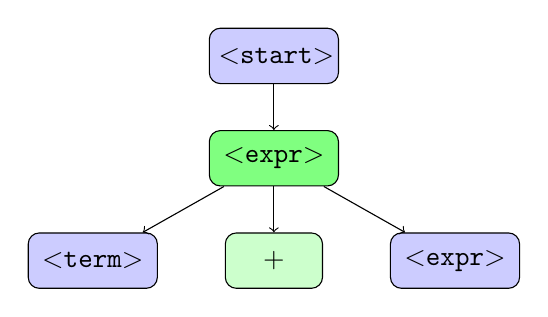
\begin{tikzpicture}[node distance=1.3cm]
  \node[bt] (s)               {\brac{start}};
  \node[bt,fill=green!50] (e0) [below of=s] {\brac{expr}};
  \node[bt,text width=1cm,fill=green!20] (+) [below of=e0] {+};
  \node[bt] (t) [left of=+,xshift=-1cm] {\brac{term}};
  \node[bt] (e1) [right of=+,xshift=1cm] {\brac{expr}};

  \path[->] (s) edge node {} (e0);
  \path[->] (e0) edge node {} (t);
  \path[->] (e0) edge node {} (+);
  \path[->] (e0) edge node {} (e1);
\end{tikzpicture}
\end{center}
This tree has the \brac{expr} \texttt{(2 * 3)} as a subtree, so
we can swap the darker green \brac{expr} we see in the above figure
with the subtree for \texttt{(2 * 3)}. Here is a tree
with that substitution carried out.
\vspace*{-1em}
\begin{center}
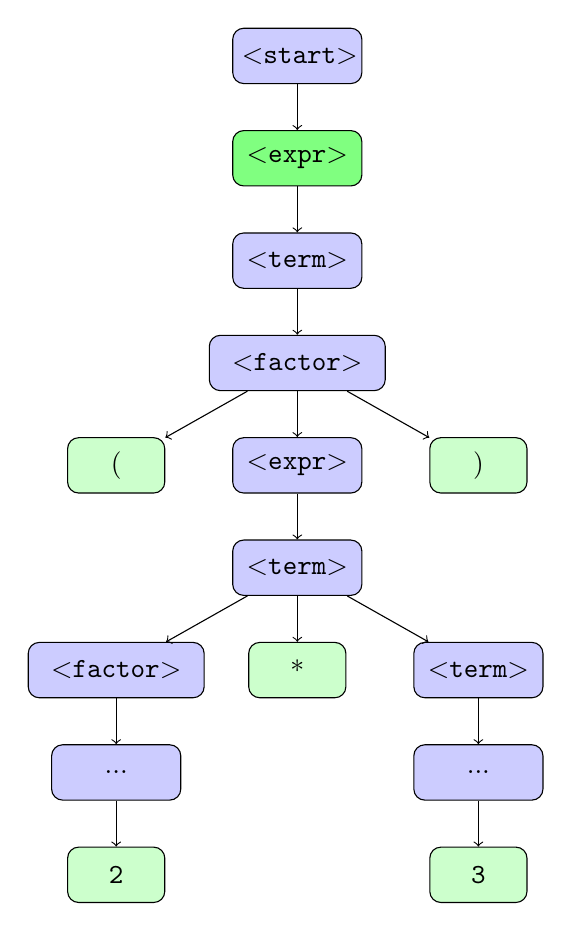
\begin{tikzpicture}[node distance=1.3cm]
  \node[bt] (s)               {\brac{start}};
  \node[bt,fill=green!50] (e0) [below of=s] {\brac{expr}};
  \node[bt] (t0) [below of=e0] {\brac{term}};
  \node[bt,text width=2cm] (f0) [below of=t0] {\brac{factor}};
  \node[bt] (e1) [below of=f0] {\brac{expr}};
  \node[bt] (t1) [below of=e1] {\brac{term}};
  \node[bt,text width=1cm,fill=green!20] (lp) [left of=e1,xshift=-1cm] {(};
  \node[bt,text width=1cm,fill=green!20] (rp) [right of=e1,xshift=1cm] {)};
  \node[bt,text width=1cm,fill=green!20] (*) [below of=t1] {*};
  \node[bt,text width=2cm] (f1) [left of=*,xshift=-1cm] {\brac{factor}};
  \node[bt] (t2) [right of=*,xshift=1cm] {\brac{term}};
  \node[bt] (f1d) [below of=f1] {...};
  \node[bt] (t2d) [below of=t2] {...};
  \node[bt,text width=1cm,fill=green!20] (2) [below of=f1d] {\texttt{2}};
  \node[bt,text width=1cm,fill=green!20] (3) [below of=t2d] {\texttt{3}};

  \path[->] (s) edge node {} (e0);
  \path[->] (e0) edge node {} (t0);
  \path[->] (t0) edge node {} (f0);
  \path[->] (f0) edge node {} (e1);
  \path[->] (f0) edge node {} (lp);
  \path[->] (f0) edge node {} (rp);
  \path[->] (e1) edge node {} (t1);
  \path[->] (t1) edge node {} (*);
  \path[->] (t1) edge node {} (f1);
  \path[->] (t1) edge node {} (t2);
  \path[->] (f1) edge node {} (f1d);
  \path[->] (t2) edge node {} (t2d);
  \path[->] (f1d) edge node {} (2);
  \path[->] (t2d) edge node {} (3);
\end{tikzpicture}
\end{center}

The relevant substituting code is:
\begin{python}
import copy
expr_input = "1 + (2 * 3)"
derivation_tree, *_ = EarleyParser(EXPR_GRAMMAR).parse(expr_input)
new_derivation_tree = copy.deepcopy(derivation_tree)
sub_expr_tree = new_derivation_tree[1][0][1][2]
new_derivation_tree[1][0] = sub_expr_tree
all_terminals(new_derivation_tree)
\end{python}
If we have the constraint that we only replace \brac{expr} nodes by
\brac{expr} nodes that are already in the tree, there is only one more
substitution we can do for the top \brac{expr}---the one that
strips the parentheses to yield unparenthesized \texttt{2*3}.
Replacing \brac{expr} nodes by non-\brac{expr} nodes will usually
violate the grammar.

\paragraph{Approach 2: Simplifying by Replacing Subtrees.}
Instead of changing like-for-like, we can change a subtree with another
alternative that is allowed by the grammar. For instance, in the tree
above, we have
\begin{verbatim}
  <term> ::= <factor> * <term>
\end{verbatim}
but, per the grammar, a \brac{term} can also be
\begin{verbatim}
  <term> ::= <factor>
\end{verbatim}
and we can modify the tree as follows:
\begin{python}
# term_tree gets "2 * 3"
term_tree = new_derivation_tree[1][0][1][0][1][0][1][1][1][0]
# shorter_term_tree gets "3"
shorter_term_tree = term_tree[1][2]  
new_derivation_tree[1][0][1][0][1][0][1][1][1][0] = shorter_term_tree
all_terminals(new_derivation_tree)
# new_derivation_tree is "(3)"
\end{python}
to yield a smaller tree, one with just a parenthesized integer \texttt{(3)}.

Our goal, then, will be to replace derivation subtrees by smaller subtrees,
and to also replace alternatives with smaller subtrees, thus simplifying
the input. Especially for structured inputs this should work much better.
But: which strategy when?

\paragraph{Implementation talk.} Once again, I'm not going to
present all of the implementation in the \emph{Fuzzing Book}.
But there is a \texttt{GrammarReducer}.

\begin{python}
class GrammarReducer(CachingReducer):
    def __init__(self, runner: Runner, parser: Parser, *,
                 log_test: bool = False, log_reduce: bool = False):
\end{python}

This class takes a \texttt{Runner} (to test inputs) and a \texttt{Parser}
(to create derivation trees from strings) and provides a couple of logging
options.

There are also some helper functions; \texttt{tree\_list\_to\_string()}
creates a string from a list of derivation trees;
\texttt{possible\_combinations()} returns the Cartesian product $\ell_1 \times \ell_2 \times \cdots$ of
the lists $\ell_1, \ell_2, \ldots$ it receives; \texttt{number\_of\_nodes()} and \texttt{max\_height()} count properties of trees.

As for the strategy implementations, \texttt{subtrees\_with\_symbol()}
is a straightforward tree traversal, not shown. 
\begin{python}
    def subtrees_with_symbol(self, tree: DerivationTree,
                             symbol: str, depth: int = -1,
                             ignore_root: bool = True) -> List[DerivationTree]:
\end{python}
It searches \texttt{tree} and returns a list of subtrees that have \texttt{symbol} at their root. We can try it out:
\begin{python}
>>> expr_input = "1 + (2 * 3)"
>>> derivation_tree, *_ = EarleyParser(EXPR_GRAMMAR).parse(expr_input)
>>> grammar_reducer = GrammarReducer(
      mystery,
      EarleyParser(EXPR_GRAMMAR),
      log_reduce=True)
>>> [all_terminals(t) for t in grammar_reducer.subtrees_with_symbol(
      derivation_tree, "<term>")]
['1', '(2 * 3)', '2 * 3', '3']
\end{python}
Because \texttt{subtrees\_with\_symbol} tells us all subtrees
that have a given symbol as root,
we can use it to look for all instances of that symbol,
which is most of the work for the substitution strategy
and also useful for finding replacements to simplify with.

The other strategy is found in \texttt{alternate\_reductions()}.
If we have a \brac{x}, and \brac{x} is defined as $Y$ or $Z$, then we
construct $Y$s and $Z$s using candidates in the tree,
and return the shortest $Y$ and the shortest $Z$ that we can construct.

This function can print all combinations making up \brac{x}. Here
we print all alternate reductions for \brac{term} in our derivation tree.
\begin{python}
>>> grammar_reducer.try_all_combinations = True
>>> print([all_terminals(t)
       for t in grammar_reducer.alternate_reductions(derivation_tree, "<term>")])
['1', '2', '3', '1 * 1', '1 * 3', '2 * 1', '2 * 3', '3 * 1', '3 * 3', '(2 * 3)', '1 * 2 * 3', '2 * 2 * 3', '3 * 2 * 3', '1 * (2 * 3)', '(2 * 3) * 1', '(2 * 3) * 3', '2 * (2 * 3)', '3 * (2 * 3)']
\end{python}
This shows all possible \brac{digit}s which are in the tree, as well as
the alternative \texttt{\brac{factor} * \brac{term}}, where it constructs
\brac{factor} and \brac{term} using components already in the derivation tree.

Without the \texttt{try\_all\_combinations} flag, it just returns the shortest
\brac{factor} and the shortest \texttt{\brac{factor} * \brac{term}}.
There is no \texttt{\brac{factor} / \brac{term}} in the tree.
\begin{python}
>>> grammar_reducer.try_all_combinations = False
>>> print([all_terminals(t)
       for t in grammar_reducer.alternate_reductions(derivation_tree, "<term>")])
['1', '1 * 1']
\end{python}

\paragraph{Combining Strategies.} We just use both strategies and deduplicate.
Despite what the comment in the code says, it's not all expansion alternatives, unless we set \texttt{try\_all\_combinations} to \texttt{True}.
\begin{python}
    def symbol_reductions(self, tree: DerivationTree, symbol: str, 
                          depth: int = -1):
        reductions = (self.subtrees_with_symbol(tree, symbol, depth=depth)
                      + self.alternate_reductions(tree, symbol, depth=depth))
        # Filter duplicates and put into unique_reductions [omitted]
        return unique_reductions
\end{python}
We can see this. Recall that a \brac{expr} is, in our case, either \texttt{\brac{term} + \brac{expr}} or just \texttt{term}.
\begin{python}
>>> print ([all_terminals(t) for t in grammar_reducer.subtrees_with_symbol(derivation_tree, "<expr>")])
['1 + (2 * 3)', '(2 * 3)', '2 * 3']
>>> print ([all_terminals(t) for t in grammar_reducer.alternate_reductions(derivation_tree, "<expr>")])
['1', '1 + (2 * 3)']
>>> print ([all_terminals(t) for t in grammar_reducer.symbol_reductions(derivation_tree, "<expr>")])
['1 + (2 * 3)', '(2 * 3)', '2 * 3', '1']
\end{python}
We can also look at potential reductions for \brac{term}. The \texttt{1 * 1} is an alternate expansion.
\begin{python}
>>> print ([all_terminals(t) for t in grammar_reducer.symbol_reductions(derivation_tree, "<term>")])
['1', '(2 * 3)', '2 * 3', '3', '1 * 1']
\end{python}

\paragraph{Overall strategy.}
There's a lot of code in the implementation of \texttt{reduce\_subtree},
but it boils down to, for each child,
(1) collecting the set of \texttt{symbol\_reductions()},
(2) checking that a reduction is indeed smaller,
and then (3) replacing the child with the reduction.
If the reduction fails (as desired), we continue by processing
the tree with the reduction in place.
The method recursively calls itself to reduce its children.

There are a bunch of helper methods, but the overall API
of the \texttt{GrammarReducer} is, as with all \texttt{Reducers},
the \texttt{reduce()} method.

\begin{python}
>>>  grammar_reducer = GrammarReducer(
       eval_mystery,
       EarleyParser(EXPR_GRAMMAR),
       log_test=True)
>>> grammar_reducer.reduce(expr_input)
Test #1 '(2 * 3)' 7 FAIL
Test #2 '2 * 3' 5 PASS
Test #3 '3' 1 PASS
Test #4 '2' 1 PASS
Test #5 '(3)' 3 FAIL
(3)
\end{python}

This does work, in 5 steps, with something that is a valid input. Indeed,
all of the tests are valid inputs, and we avoid the \texttt{UNRESOLVED}
parse errors.

\paragraph{Adding depth.} So far, we try to replace subtrees with
the smallest possible subtrees; we replace \texttt{2 * 3} by first
\texttt{2} and then \texttt{3}. Going straight to small trees may remove too much at once, and delta debugging
tries to remove a ``sensible'' amount at once. In the tree context, we want to replace
with larger subtrees instead of the smallest possible subtree.

How do we get larger subtrees? We replace by subtrees that are closer
to the root, i.e. that have smaller depth. By definition, they are larger.

The \texttt{subtrees\_with\_symbol()} function can take a \texttt{depth}
parameter, which makes it only return subtrees at the given depth.

The example in the \emph{Fuzzing Book} doesn't completely make sense to me,
but the search starts with depth 0 and increases it. So, we preferentially
replace with bigger subtrees.

We can observe the behaviour:
\begin{python}
>>>  grammar_reducer = GrammarReducer(
       eval_mystery,
       EarleyParser(EXPR_GRAMMAR),
       log_test=True)
>>> grammar_reducer.reduce_tree = grammar_reducer.reduce_tree_with_depth
>>> grammar_reducer.reduce(expr_input)
Test #1 '(2 * 3)' 7 FAIL
Test #2 '(3)' 3 FAIL
Test #3 '3' 1 PASS

'(3)'
\end{python}
The key differences are that this doesn't try the subtrees
\texttt{2 * 3}, or the single-digit subtrees. It replaces the entire
\brac{expr} with the \texttt{(2 * 3)} \brac{expr}, as before.
Then, it replaces the remaining \brac{term} by the \brac{factor}
that goes to the \brac{digit} 3. There is nothing more that fails,
so it terminates. This terminates in 3 steps instead of 5.

\section*{Grammar-Based versus Delta Debugging}
Let's measure effectiveness. Here is a long expression:

\begin{python}
long_expr_input = GrammarFuzzer(EXPR_GRAMMAR, min_nonterminals=100).fuzz()
\end{python}

And we can use the grammar reducer:
\begin{python}
grammar_reducer = GrammarReducer(eval_mystery, EarleyParser(EXPR_GRAMMAR))
with Timer() as grammar_time:
    print(grammar_reducer.reduce(long_expr_input))
\end{python}
I ran it and it needed 9 tests, finishing in 0.033s.

versus the delta debugger:
\begin{python}
dd_reducer = DeltaDebuggingReducer(eval_mystery)
with Timer() as dd_time:
    print(dd_reducer.reduce(long_expr_input))
\end{python}
This took 618 tests and took 0.503s.

We can see that where there is a grammar, the grammar reducer wins handily.

\end{document}
